\documentclass[thesis.tex]{subfiles}

\begin{document}

\chapter{Background and Motivation}
\label{cha:background}

In this chapter, we first show the trends of swarm applications and how they
differ from previous topics, such as wireless sensor networks, cyber-physical
systems and ubiquitous computing. By analyzing the fundamental properties of
swarm applications, we summarize the core challenges with developing swarm
applications, such as constrained resources and heterogeneous environment.

One key potential with swarm applications is due to the scale facilitated by the
inter-connectivity, especially as the cloud becomes mature and is used as the
universal computation and storage backend. Many applications are constructed by
directly connecting devices to the cloud. This trend, although understandable,
is not the best long term approach. We discuss the pitfalls with this
cloud-centric approach and argue that ``the cloud is not enough.''

To accompany the cloud, a new tier of computing infrastructure, the edge,
arises. Due to their close proximity to end devices, the edge is effective to
reduce network latency and provide more resource guarantees to end
devices. However, unlike the cloud, the edge is resource constrained and it is
unclear what capabilities we can expect from the edge. As a result, swarm
applications relying on the edge need to take the heterogeneous landscape into
account.

\section{The Emerging Swarm}
\label{sec:emerging-swarm}

Smart devices are everywhere: \href{http://ilumi.co/}{light bulb},
\href{https://nest.com/}{thermostat}, \href{http://lunasleep.com/}{mattress
  cover}, \href{https://www.indiegogo.com/projects/smart-diapers}{e-diaper},
\href{https://www.fitbit.com/}{fitness tracker},
\href{https://www.fitbit.com/aria}{smart scale},
\href{https://www.myvessyl.com/}{smart cup},
\href{https://www.kickstarter.com/projects/1816678675/smartplate-instantly-track-and-analyze-everything}{smart
  plate},
\href{http://www.amazon.com/HAPILABS-102-HAPIfork-Bluetooth-Enabled-Smart/dp/B00FRPCPEC}{smart
  fork}, \href{http://electroluxdesignlab.com/en/submission/smart-knife/}{smart
  knife},
\href{http://www.clickandgrow.com/pages/what-is-click-grow}{flowerpot},
\href{http://www.williams-sonoma.com/products/breville-die-cast-2-slice-stainless-steel-smart-toaster/}{toaster},
\href{https://garageio.com/}{garage door},
\href{http://www2.withings.com/us/en/products/baby/smart-baby-monitor}{baby
  monitor},
\href{https://www.indiegogo.com/projects/smartmat-the-world-s-first-intelligent-yoga-mat}{yoga
  mat},
\href{http://usnews.rankingsandreviews.com/cars-trucks/best-cars-blog/2013/02/2015_GM_Vehicles_Will_Get_Wi-Fi_Internet_Access/}{sport-utility
  vehicle}, and
\href{http://www.samsung.com/us/appliances/refrigerators/RF28HMELBSR/AA}{refrigerator}.\footnote{Courtesy
  of Prof.\,Randy Katz.} Capable of computation and communication, they monitor
and interact with the physical world.  The growth of number of devices is
staggering: analysts predicted 26 billion devices by 2020 and trillion by
2022~\cite{middleton2013forecast}.

We refer to the collection of sensors and actuators installed in our environment
as the ``Swarm'', a term coined by Jan Rabaey during a keynote talk at ASPDAC
2008~\cite{rabaey2008brand}. This term well characterizes where the potentials
lie: it is not in the individual components, but rather the scale and the number
of interconnected devices, a shift from Moore's Law\footnote{The number of
  transistors on a chip doubles about every two years at the same cost.} to
Metcalfe's Law.\footnote{The effect of a telecommunications network is
  proportional to the square of the number of connected users of the system,
  i.e., $n^2$.}

At Berkeley, the Qualcomm Ubiquitous Swarm Lab~\cite{swarmlab} and Terraswarm
Research Center~\cite{terraswarm} were launched to address the huge potentials
and challenges for Swarm systems in December 2011 and January 2013,
respectively. Outside of Berkeley, this trend is also gaining attraction,
although the names can be different: Internet of Things
(IoT)~\cite{atzori2010internet}, Internet of Everything
(IoE)~\cite{bradley2013internet}, Industry 4.0~\cite{lasi2014industry}, The
Industrial Internet~\cite{eigner2018industrial}, Trillion Sensors
(TSensors)~\cite{bogue2014towards}, Machine to Machine
(M2M)~\cite{anton2014machine}, Smarter Planet~\cite{palmisano2008smarter}, etc.

Due to the widespread use of ``IoT'' outside of Berkeley, we use ``IoT'' and
``swarm'' interchangeably throughout this thesis. However, ``swarm'' is
preferred, because, quoting Lee~\cite{lee2016iot},

\begin{displayquote}
  The term ``IoT'' includes the technical solution ``Internet technology'' in
  the problem statement ``connected things.''
\end{displayquote}

\subsection{Swarm Applications}
\label{sec:swarm-applications}

With billions of devices interconnected, the swarm makes a large number of
applications possible. A previous survey by Atzori et al.\, groups applications
based on their domains: 1) transportation and logistics; 2) health-care domain;
3) smart environment (home, office, plant); 4) personal and
social~\cite{atzori2010internet}. We characterize the applications based on the
usage pattern. In this way, it is easier to analyze application requirements and
understand implications for system support. We characterize swarm applications
into two general categories.\footnote{Note that these two categories are not
  exclusive to each other. Some applications may fall into both.}

\subsubsection{Ambient Data Collection and Analytics}
\label{sec:ambi-data-coll}

A wide range of swarm applications collect sensor data and monitor our
environment. They operate at vastly different scales:
cities~\cite{cheng2014aircloud, sfpark}, buildings~\cite{dawson2010smap},
homes~\cite{hnat2011hitchhiker}, and individuals (also referred to as Quantified
Self)~\cite{fitbit, swan2013quantified}. Because of the close interaction with
our environment, these applications often have a direct impact on our everyday
life and can help solve societal-scale problems. For example, in metropolitan
cities in developing countries, such as Beijing, the air quality has
deteriorated significantly. Air quality monitoring with fine granularity can
advise people with appropriate actions such as wearing masks or stay at
home~\cite{cheng2014aircloud}.

Many environmental sensors are collecting data about physical properties that
are intrinsically slow-changing, such as the occupancy, temperature, humidity,
etc. As a result, these sensors sample at low frequency (millihertz, i.e.,
slower than 1 Hz). For example, in a campus-wide building instrumentation that
aims to reduce energy usage~\cite{krioukov2012building}, there are 2,151
\href{http://www.keti.re.kr/}{KETI Motes}---463 \ce{CO2} sensors, 466 humidity
sensors, 26 illumination sensors, 440 light sensors, 290 PIR (passive infrared)
sensor, and 466 temperature sensors---configured to report data every five
seconds. For the air quality monitoring mentioned above, the sensors only sample
once a minute.

On the other hand, we are seeing high-frequency, high-precision sensors being
deployed at scale as technology evolves and applications' requirement
changes. For example, energy disaggregation takes a whole building's aggregated
energy signal and separates it into appliance-specific data. Recent works start
to sample at 15 kHz or higher to analyze the harmonics to identify type of
electrical circuitry in appliance~\cite{kolter2011redd} with a higher
accuracy. This contrasts with prior approaches using low sampling rates and only
relying on state changes~\cite{hart1992nonintrusive}.

Regardless of the sampling frequency and data rate, in this category,
applications do not inspect the data immediately and often store it for future
analytics and archival purposes. Data scientists may employ exploratory data
analysis to visualize the collected data for patterns, or compare data across
sensors and time for insights.

The aggregated historical data will keep increasing and create a new kind of
big-data problem~\cite{diaz2012big, zaslavsky2013sensing}, challenging our
existing ways of data storage and analysis. For example, microsynchophasors, or
uPMUs, monitor the electrical grid with a network of 1000 devices; each produces
12 streams of 120 Hz high-precision values accurate to 100 ns. This amounts to
1.4 million points per second and requires specialized storage systems for
time-series analysis~\cite{andersen2016btrdb}.

At last, because the collected data can be related with personal health or
manufacture's operation status, many of these applications have serious privacy
implications.

\subsubsection{Real-time Applications with Low-Latency Requirements}
\label{sec:inter-low-latency}

Interactive applications that involve humans in the loop require a low latency
response to engage the users. For example, Wearable cognitive
assistant~\cite{chen2018application} uses wearable devices, such as Google
Glass, for deep cognitive assistance (e.g., offering hints for social
interaction via real-time scene analysis). A general rule of thumb for systems
that give the feeling of instantaneous response is to bound the latency to 100
ms~\cite{miller1968response, nielsen1994usability}.

In autonomous systems where humans are not involved, a tight control over
latency is important for proper and deterministic
behavior~\cite{eidson2012distributed}, especially when it involves a group or
feedback control. Schulz et al.~\cite{schulz2017latency} summarizes several
latency critical uses, including factory automation, smart grids, intelligent
transport systems, etc.

Satisfying applications' tight latency requirements is challenging. Timing
behavior in software execution emerges from implementations rather than
specifications~\cite{lee2018real}. The goal for timing is often to speed up some
execution, but not to provide guaranteed and repeatable timing. Similarly, the
Internet provides ``best-effort'' service and fails to provide quality of
service (QoS) guarantees~\cite{shenker1995fundamental}. The situation is
becoming worse as swarm applications become more complex and generate large
amount of data.

\subsection{Heterogeneous Swarm Platforms}
\label{sec:swarm-platforms}

There has been a dizzying array of embedded platforms, from powerful computing
units to low-power microcontrollers (see \autoref{tab:embedded}).

\subsubsection{Microcontrollers}

Examples include Arduino~\cite{arduino}, mbed~\cite{mbed}, and
Spark~\cite{spark}. This emerging category continues to expand as new open
platforms appear on crowdfunding websites~\cite{kickstarter}.  With an
ecosystems featuring great support and libraries (e.g., Adafruit Online
Tutorials~\cite{adafruit}), people can easily add new sensors/actuators and
develop applications. These platforms have unleashed the creativity of millions
in building smart and interactive devices, spawning the Maker
Movement~\cite{dougherty2012maker}.

\subsubsection{Smartphones}

As a key enabler for mobile computing, smartphones have become ubiquitous. They
are equipped with an impressive set of sensors, including accelerometer,
gyroscope, proximity sensor, camera, microphone, etc. The processors and
displays on smartphones keep upgrading. In addition to use smartphones alone,
many companies (like Fitbit~\cite{fitbit} or Automatic~\cite{automatic}) use
smartphones as gateways to connect low-power devices to the Internet via
Bluetooth. Creative use of smartphones is also a hot topic in research,
including reusing discarded smartphones~\cite{challen2014mote}, writing new
operating systems~\cite{janos}, and developing novel
applications~\cite{hong2014smartphone}.

\subsubsection{Mini PCs}

Ranging from powerful Intel Next Unit of Computing (NUC) to inexpensive
Raspberry Pi, BeagleBone Black, these devices typically run various versions of
Linux to simplify application deployment. Many companies~\cite{ninja,
  smartthings, wink} adopt these mini PCs with all kinds of networking
capabilities---802.15.4, Bluetooth, WiFi, Ethernet---as their gateway devices.
In contrast to using smartphones as gateways, mini PCs serve as nearby
always-available infrastructure---the ``immobiles.''~\cite{swarmbox}.

\begin{table}
  \centering
  \begin{tabular}{c c c c}
    \toprule
    Device & CPU Speed & Memory & Price \\
    \midrule
    Intel NUC & 1.3 GHz & 16 GB & \texttildelow\$300 \\
    Typical Phones & 2 GHz & 2 GB & \texttildelow\$300 \\
    Discarded Phones\tablefootnote{This data is from \cite{challen2014mote}, where the
    original authors noted ``Customer buyback price quoted by Sprint for a
    smartphone in good condition.''}
           & 1 GHz & 512 MB & \texttildelow\$22 \\
    BeagleBone Black & 1 GHz & 512 MB & \$55 \\
    Raspberry Pi & 900 MHz & 512 MB & \$35 \\
    Arduino Uno & 16 MHz & 2 KB & \texttildelow\$22 \\
    %% http://arduino.cc/en/Products.Compare
    mbed NXP LPC1768 & 96 MHz & 32 KB & \$10 \\
    \bottomrule
  \end{tabular}
  \vspace*{-0.075in}
  \caption{The swarm includes a wide spectrum of computing platforms (price as
    of 2015).}
  \vspace*{-0.1in}
  \label{tab:embedded}
\end{table}

%% CSV Data:
%% Intel NUC:
%% http://www.intel.com/content/dam/www/public/us/en/documents/product-briefs/nuc-kit-d54250wyk-product-brief.pdf

% Platform, CPU, Memory, Price
% Intel NUC, 1.3 GHz*4, 16 GB,
% Apple A8, 1.4 GHz*2, 1 G, $600
% Nexus 6, 2.7 GHz*4, 3G, $600
% Raspberry Pi, 900MHz*4, 1G, $35
% BeagleBone, 720MHz, 256MB,
% Arduino, 16MHz, 8KB, $75
% mbed NXP LPC11U24, 48MHz, 8KB, $10
% mbed NXP LPC1768, 96MHz, 32KB, $10

\subsection{Swarm and Related Concepts}
\label{sec:swarm-relat-conc}

At first glance, the swarm may seem similar to other concepts such as wireless
sensor network (WSN), cyber-physical systems (CPS), and ubiquitous computing
(Ubicomp). In this section, we will show the difference with side-by-side
comparisons. We argue that the swarm has its fundamental differences and new
challenges to address.

\subsubsection{Swarm and WSN}
\label{sec:swarm-wsn}

In the 1990s, ``Smart Dust''~\cite{kahn1999next} envisions wireless sensor nodes
with a volume of one cubic millimeter that can sense, communicate and
compute. Being so small, these devices can then be spread through our
environment and enhance our interaction with the physical world. This vision
quickly leads to deploying a group of spatially dispersed and dedicated wireless
sensors---a wireless sensor network---to monitor and record the physical
conditions of the environment

WSNs offer the potential to dramatically advance scientific fields or extracting
engineering insights with dense temporal and spatial measurements. Without
exhaustively listing the rich literature~\cite{akyildiz2002wireless,
  zhao2009wireless}, we show a few notable deployments as follows,

\begin{itemize}[itemsep=5pt]
\item \textbf{ZebraNet}~\cite{zhang2005habitat}. Zhang et al.\, deployed 7 nodes
  by placing sensor nodes into the zebra's collar at the 24,000-acre Sweetwaters
  Reserve at Kenya. The nodes traveled with zebras and measuresd GPS positions
  and sun/shade indication.
\item \textbf{Redwoods}~\cite{tolle2005macroscope}. Tolle et al.\,deployed 80
  nodes at the redwoods in Sonoma, California. The network recorded 44 days of
  air temperature, relative humidity, and photosynthetically active solar
  radiation data.
\item \textbf{GGB}~\cite{kim2007health}. Kim et al.\,deployed 59 nodes over the
  span and the tower of the Golden Gate Bridge. The network collected ambient
  vibrations in two directions synchronously at 1 kHz rate for structural health
  monitoring.
\end{itemize}

We then compared the swarm with WSNs and show that while the swarm finds its
origin in the WSN concept, the swarm represents a much broader vision,
potentially connecting trillions of sensory and actuating devices that are
heterogeneous and worldwide into a single platform abstraction.

\para{WSN is application-specific; the swarm can re-purpose itself}. Most WSNs
focus on specific use cases. Because energy is usually the primary concern in
deployed networks, the lifespan of a network benefits greatly from custom
hardware design and careful tuning of software stack. After the deployment,
sensor nodes are dedicated for the particular task. For the swarm, it is
important to be reprogrammed on the fly for other purposes. This is best
illustrated with the vision of ``a tale of two smart
cities''~\cite{lee2012terraswarm}: the swarm allows safe, efficient, and
comfortable transportation and communication during the best of times, and
secure, quick, and adaptable emergency response during the worst of times. The
swarm is more efficient through sharing of resources; it is more resilient
through dynamic recruiting; and it is more capable by enabling novel
applications beyond developers' imagination. At the same time, the open
architecture can lead to bigger security and privacy risks.

\para{WSN nodes are significantly less heterogeneous than swarm devices}. WSNs
typically are comprised of sensor nodes and gateway nodes. Sensors nodes are
often the same batch of hardware and form a star, tree or mesh network after
deployment. Gateway nodes are more powerful in processing capability, battery
life, and transmission range, acting as data aggregation point and bridge to
other networks. In comparison, each swarm node can have different types of
sensors and actuators. Their processing and networking capabilities will depend
on many factors, including tasks, prices, manufactures and hardware
availability.

\para{WSNs are mostly stand-alone while the swarm interacts with the cloud and
  others closely}. Once deployed, WSNs rarely interact with the external world,
except shipping sensor data to some central storage location via the
gateways. Therefore, when designing WSN, one has to carefully provision the
resources. The swarm, on the other hand, coexists and closely interacts with the
cloud and other essential components of the Internet. The cloud offers unbounded
computational, communication and storage capacity. By offloading tasks to the
cloud, the swarm can achieve what is beyond its own hardware capability.

\subsubsection{Swarm and CPS}
\label{sec:swarm-cps}

Cyber-physical systems (CPS), coined by Helen Gill in 2006, refers to the
integration of computation (the cyber) and physical processes (the
physical)~\cite{lee2015past}. CPS applications include industrial automation,
manufacturing, transportation, medical devices, energy systems, and distributed
robotics.

Because ``cyber'' and ``physical'' parts are tightly coupled in a feedback
relation, it is important to study the intersection, or the joint dynamics, of
the two for a complete understanding of the systems~\cite{rajkumar2010cyber}. It
is not sufficient to separately understand only one side. For example, for many
applications only in the cyberspace, i.e., general-purpose software, timing is a
performance concern: a slower program is not an incorrect program and reducing
the execution time is a performance optimization. In CPS, because the decision
made by the cyber parts affect the physical processes and subsequent feedback
reactions, a precise control of the timing is often a correctness
concern. Another challenge that is unique in the intersection of ``cyber'' and
``physical'' is the level of concurrency. Physical processes are composed of
many parallel processes. Software, on the other hand, is often constructed as a
sequence of steps. The challenge is to bridging the inherent sequential cyber
world with the concurrent physical world.

One can view the swarm as a realization of CPSs: in addition to the timing and
concurrency challenges, the swarm emphasizes the concept of intensively
networked components. Leveraging Internet technology to connect and
unprecedented number of devices, yielding a ``swarm'' of heterogeneous sensors
and actuators that can interact with the physical environment and can be used to
enable dynamic decision making in many different domains. 

Swarm challenges in addition to CPS. This ability builds upon the implicit
assumption that systems will be able to make real-time decisions on streaming
data. While the meaningful interpretation of this specification is exceedingly
context-dependent, for the purposes of the IoT, the implied requirement is the
ability of a system to contin- ually process streams of data in order to extract
actionable information.

\subsubsection{Swarm and Ubicomp}
\label{sec:swarm-wsn}

What is Ubicomp? Ubiquitous computing (or ``ubicomp'') is a concept in software
engineering and computer science where computing is made to appear anytime and
everywhere.

Swarm and Ubicomp.

Swarm challenges.

%%% Local Variables:
%%% mode: latex
%%% TeX-master: "../background"
%%% End:

\section{Massive Adoption of Cloud Platforms}
\label{sec:cloud}

Over the last few years, cloud computing has shaped the software industry and
made the development and deployment of web services easier than ever.  Public
cloud providers such as Amazon, Microsoft, Google, Rackspace offer pay-as-you-go
services for the general public.  Such a service model has reduced capital
expenses, enabled elasticity for dynamic load adaption, and simplified resource
management~\cite{armbrust2010view}.

We have seen a huge recent trend of migrating computations and services to the
cloud.  Taking Amazon S3 as an example, over two trillion objects were reported
stored in the system back as of April 2013~\cite{barr2013amazon}.  Riding on
this popularity, application developers in the IoT space have blithely adopted
the cloud as a universal computation and storage backend.  This approach has
been taken by both industrial efforts (such as Carriots~\cite{carriots},
GroveStreams~\cite{grovestreams}, SAMI~\cite{sami}, Xively~\cite{xively}) and
academic research~\cite{gupta2014bolt, zachariah1001internet}.

%%% Local Variables:
%%% mode: latex
%%% TeX-master: "../background"
%%% End:

\section{The Cloud is Not Enough}
\label{sec:cloud-not-enough}

Riding on this popularity of the cloud, many of today's IoT solutions arise by
connecting embedded platforms to the cloud as a universal computation and
storage backend. This approach has been taken by both industrial efforts (such
as Carriots~\cite{carriots}, GroveStreams~\cite{grovestreams}, SAMI~\cite{sami},
Xively~\cite{xively}) and academic research~\cite{gupta2014bolt,
  zachariah1001internet}. For example, Bolt~\cite{gupta2014bolt} provides data
management for the Lab of Things (LoT)~\cite{brush2013lab} and uses Amazon S3 or
Azure for data storage. Such direct connections often require an application
gateway~\cite{zachariah1001internet} to support low-power wireless
communications such as Z-Wave or Bluetooth Low Energy (BLE).

The IoT industry has benefited hugely from the economic model of the cloud.
With little investment in infrastructure, even novice users can start collecting
sensor data and streaming it back to the cloud~\cite{armbrust2010view}.  Several
IoT cloud platforms~\cite{carriots, grovestreams, xively, sami} have gone
further by offering easy-to-use APIs, data processing, visualization, and sample
code for various hardware platforms.

At first glance, directly using the cloud seems to be a natural architecture for
swarm applications. However, several significant problems with this approach are
revealed on closer inspection, including issues with privacy, security,
scalability, latency, bandwidth and availability.  While these problems are not
new to typical web applications, they are exacerbated in the swarm space because
of fundamental differences between swarm and web services. Our reasoning is as
follows:

\begin{table}
  \centering
  \begin{tabular}{c c c}
    \toprule
    & Web/IT & Swarm/IoT \\
    \midrule
    Privacy \& Security & Open for access & Sensitive data \\
    Scalability & Power law & Billion devices \\
    Interaction Model & Human & Machine \\
    Latency & Variable & Bounded  \\
    Bandwidth & Downstream & Upstream   \\
    Availability (QoS) & No guarantee & Requirement  \\
    Durability Management & Cloud controls & Users control \\
    \bottomrule
  \end{tabular}
  \caption{Pitfalls with Today's Approach to directly using the cloud.}
\end{table}

\begin{enumerate}

\item \textbf{Privacy and Security.} Sensors implanted in our surrounding
  environment collect extremely sensitive information.  In a recent talk given
  by Wadlow~\cite{wadlow}, he described the IoT as ``hundreds of computers that
  are aware of me, can talk about me, and are out of my control.''  This is a
  strong call for intrinsic security and privacy.  This need is echoed in
  critical posts and talks---``Internet of Crappy
  Things''~\cite{alex2015internet}, ``The Internet of
  Fails''~\cite{stanislav2014the}, etc.  The FTC's Technical
  Report~\cite{ftc2015internet} also emphasizes security in the IoT spaces.  As
  a centralized resource out of users' control, the cloud presents an
  ever-present opportunity to violate privacy.  Today, privacy has become a
  luxury~\cite{angwin2014has}, a situation that will be exacerbated in the IoT.

\item \textbf{Scalability.} By 2020, Cisco estimates 50
  billion~\cite{evans2011internet} devices will be connected to the cloud, while
  Gartner estimates 26 billion~\cite{middleton2013forecast}. Scalability in the
  IoT spaces will be more challenging than web-scale or Internet-scale
  applications; the amount of data generated easily exceeds the reported
  trillion objects in Amazon S3~\cite{barr2013amazon}. The bisection bandwidth
  requirements for a centralized cloud solution are staggering, especially since
  most data acquired by IoT devices can or should be processed locally and
  discarded.

\item \textbf{Modeling: Peripheral devices are physical.}  Both sensors and
  actuators are physically present devices in our environment.  Although sensor
  data can be collected and replicated (similar to virtualizing
  sensors~\cite{yuriyama2010sensor}), the data is still generated from the edge
  of the network.  Moreover, actuators cannot be virtualized and oftentimes the
  actuations cannot be rolled back.  This is significantly different from the
  model of web services today.

\begin{figure}
  \centering
  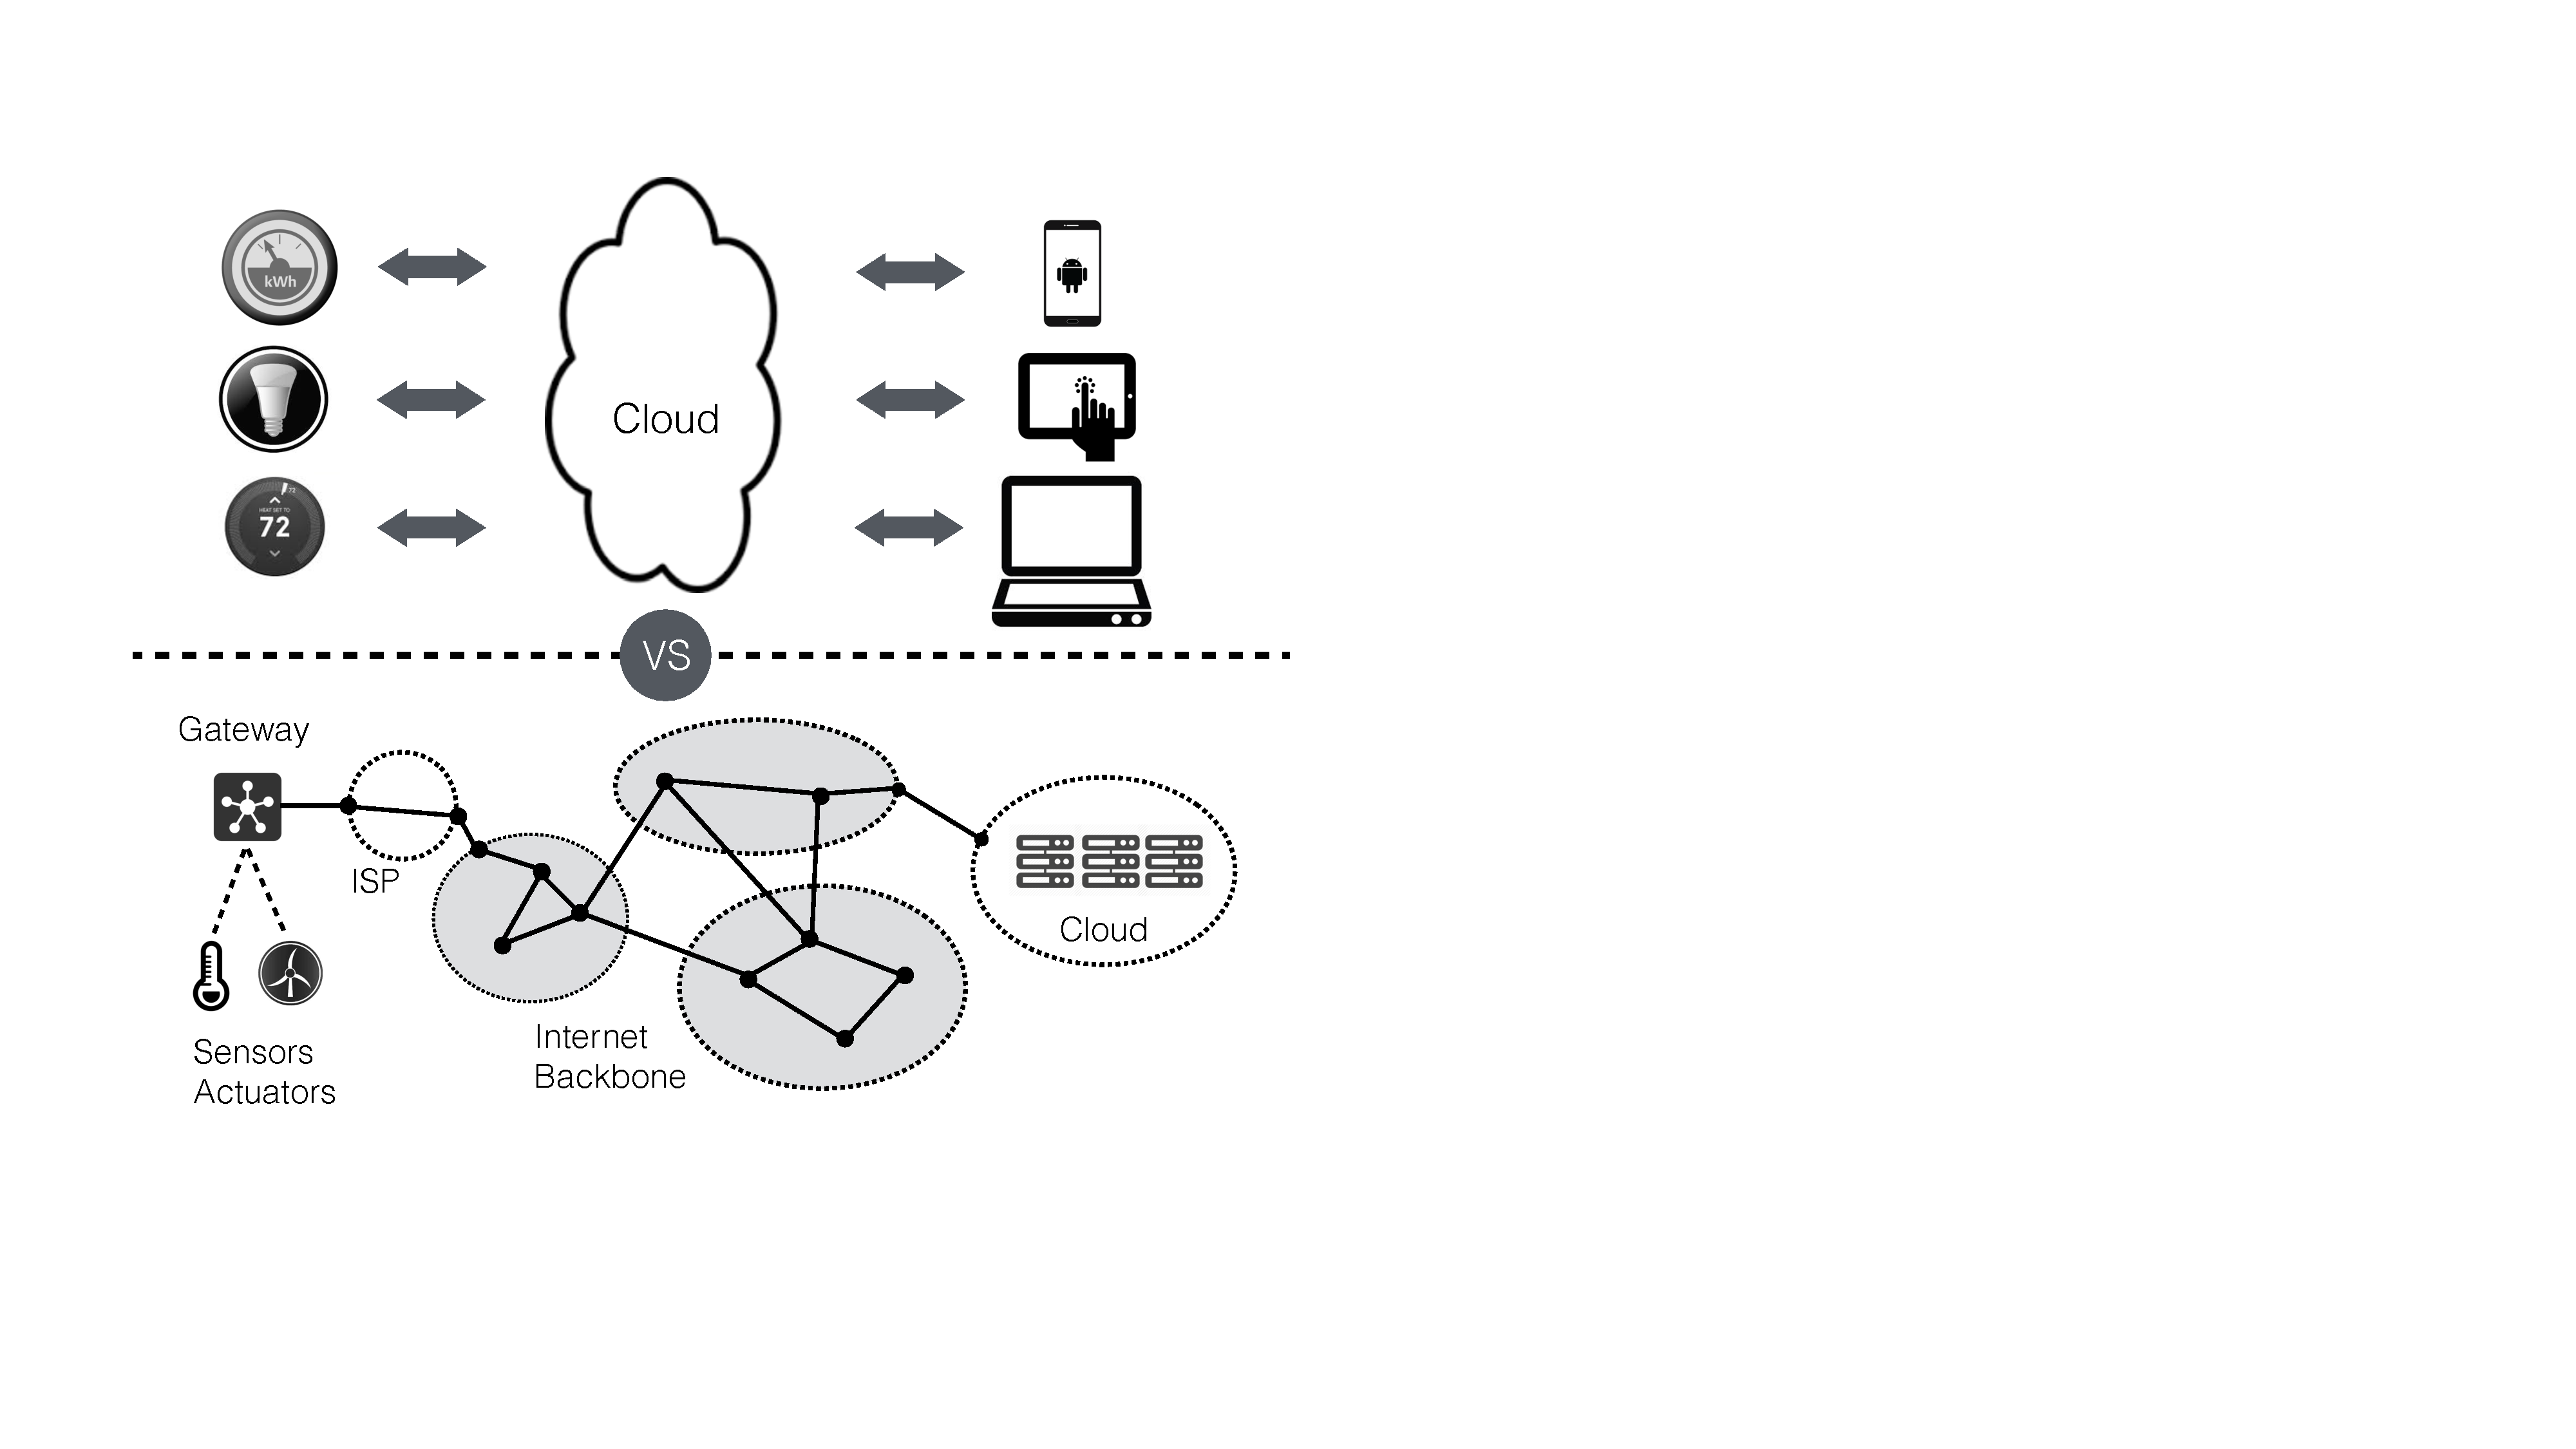
\includegraphics[width=0.6\columnwidth]{figures/cloud-view.pdf}
  \caption{Although applications usually view the cloud as the center of
    all connected devices (\textit{upper diagram}), in reality the cloud
    is usually on the edge of the Internet backbone, just like other
    devices (\textit{lower diagram}).}
  \label{fig:network}
\end{figure}

\item \textbf{Latency: The cloud model differs from reality.}  Application
  developers view the cloud as a component that interconnects the smart devices.
  However, from a network point of view, the cloud is on the edge of the network
  (see \autoref{fig:network}).  Even simple IoT applications, such as those that
  turn on a fan in response to a rise in local temperature, will experience
  unpredictable latencies from sensing, wireless transmission, gateway
  processing, Internet Service Provider (ISP), Internet, and cloud processing.

%% - sensor latency: 10-100 microseconds
%% - wireless latency: 676 µs (BLE, Overview and Evaluation of Bluetooth Low
%% Energy: An Emerging Low-Power Wireless Technology). Normally it's ~100 ms.
%% May need some data from http://iplane.cs.washington.edu/data/data.html

\item \textbf{Bandwidth: Upstream traffic dominates.}  Shipping data to the
  cloud incurs a significant amount of upstream traffic.  Typical broadband
  networks have more downstream bandwidth than upstream bandwidth.  IoT
  applications, however, generate data at the edges of the network, a pattern
  that will easily saturate the upstream link bandwidth---especially at scale.
  For example, a single Dropcam requires ``a high speed internet connection with
  at least 0.5 Mbps'' to use its service~\cite{dropcam}.  Even simple sensors,
  such as energy meters, can benefit from a higher sampling rate (the motivation
  of 1 kHz energy data with ground-truth from the Ubicomplab at the University
  of Washington~\cite{gupta2015household} and 15 kHz sampling of energy from MIT
  REDD Dataset~\cite{kolter2011redd}).

\item \textbf{Quality of Service (QoS) Guarantees.} Web users tolerate
  variable latency and occasional loss of web services.  In contrast, the
  temporary unavailability of sensors or actuators within IoT applications will
  directly impact the physical world.  While significant engineering effort has
  been put into improving the availability and latency profile of the cloud
  (allowing Service Level Agreements), such efforts are stymied by operator
  error, software bugs, DDoS attacks, and normal packet-to-packet variations
  from wide-area routing. Further, the Internet connection to people's homes is
  far from perfect.  Over 10\% of home networks in the developed world see
  connectivity interruptions of more than ten minutes more frequently than once
  every 10 days~\cite{grover2013peeking}; this situation is worse in developing
  countries.

\item \textbf{Durability Management.} Some sensor data is ephemeral: while other
  data should be durable against global disasters.  For ephemeral data, there is
  no effective way of verifying the data has been completely destroyed because
  the cloud is out of the user's control. For durable data, regardless of the
  promised guarantees~\cite{s3durability}, the reliability of cloud storage
  remains a major concern and there is active research in this
  direction~\cite{bessani2013depsky}.  Moreover, whatever durability is achieved
  by the cloud, it is typically done so without concern for application-specific
  privacy or export rules.  Note that control over durability is closely related
  to control in general: making sure that users retain control over their data
  rather than providers.

\end{enumerate}

%%% Local Variables:
%%% mode: latex
%%% TeX-master: "../background"
%%% End:

\section{Edge Computing}
\label{sec:edge-computing}

The edge represents a new tier of infrastructure envisioned to address some of
the pitfalls with the cloud for IoT applications. Cisco named it \textit{the
  fog} because the fog is a cloud close to the ground~\cite{bonomi2012fog}. CMU
chose \textit{cloudlet} to indicate this small-scale cloud
datacenter~\cite{ha2014towards, satyanarayanan2009case}. At Berkeley, we use
\textit{swarmbox} to name the hardware platform that accompanies swarm
devices. Both Smartphones and Mini PCs mentioned
in~\autoref{sec:swarm-platforms} can act as edge computing platforms. Other edge
computing infrastructure may be provided by carriers, hosted in central
offices\footnote{Often, a central office is defined as a building used to house
  the inside plant equipment of potentially several telephone exchanges, each
  serving a certain geographical area.} or cell towers~\cite{att2017edge}.

One common form of the edge computers are gateways. Many gateways provide
application-specific connectivity for IoT devices to interact with the Internet,
bridging low-power communication protocols such as BLE/802.15.4 to IP. Even when
devices can utilize more standard communication protocols such as WiFi, the
gateways still exist as downloadable applications that run on cellphones or
computers, providing custom services or user interfaces.

\begin{figure}
  \centering
  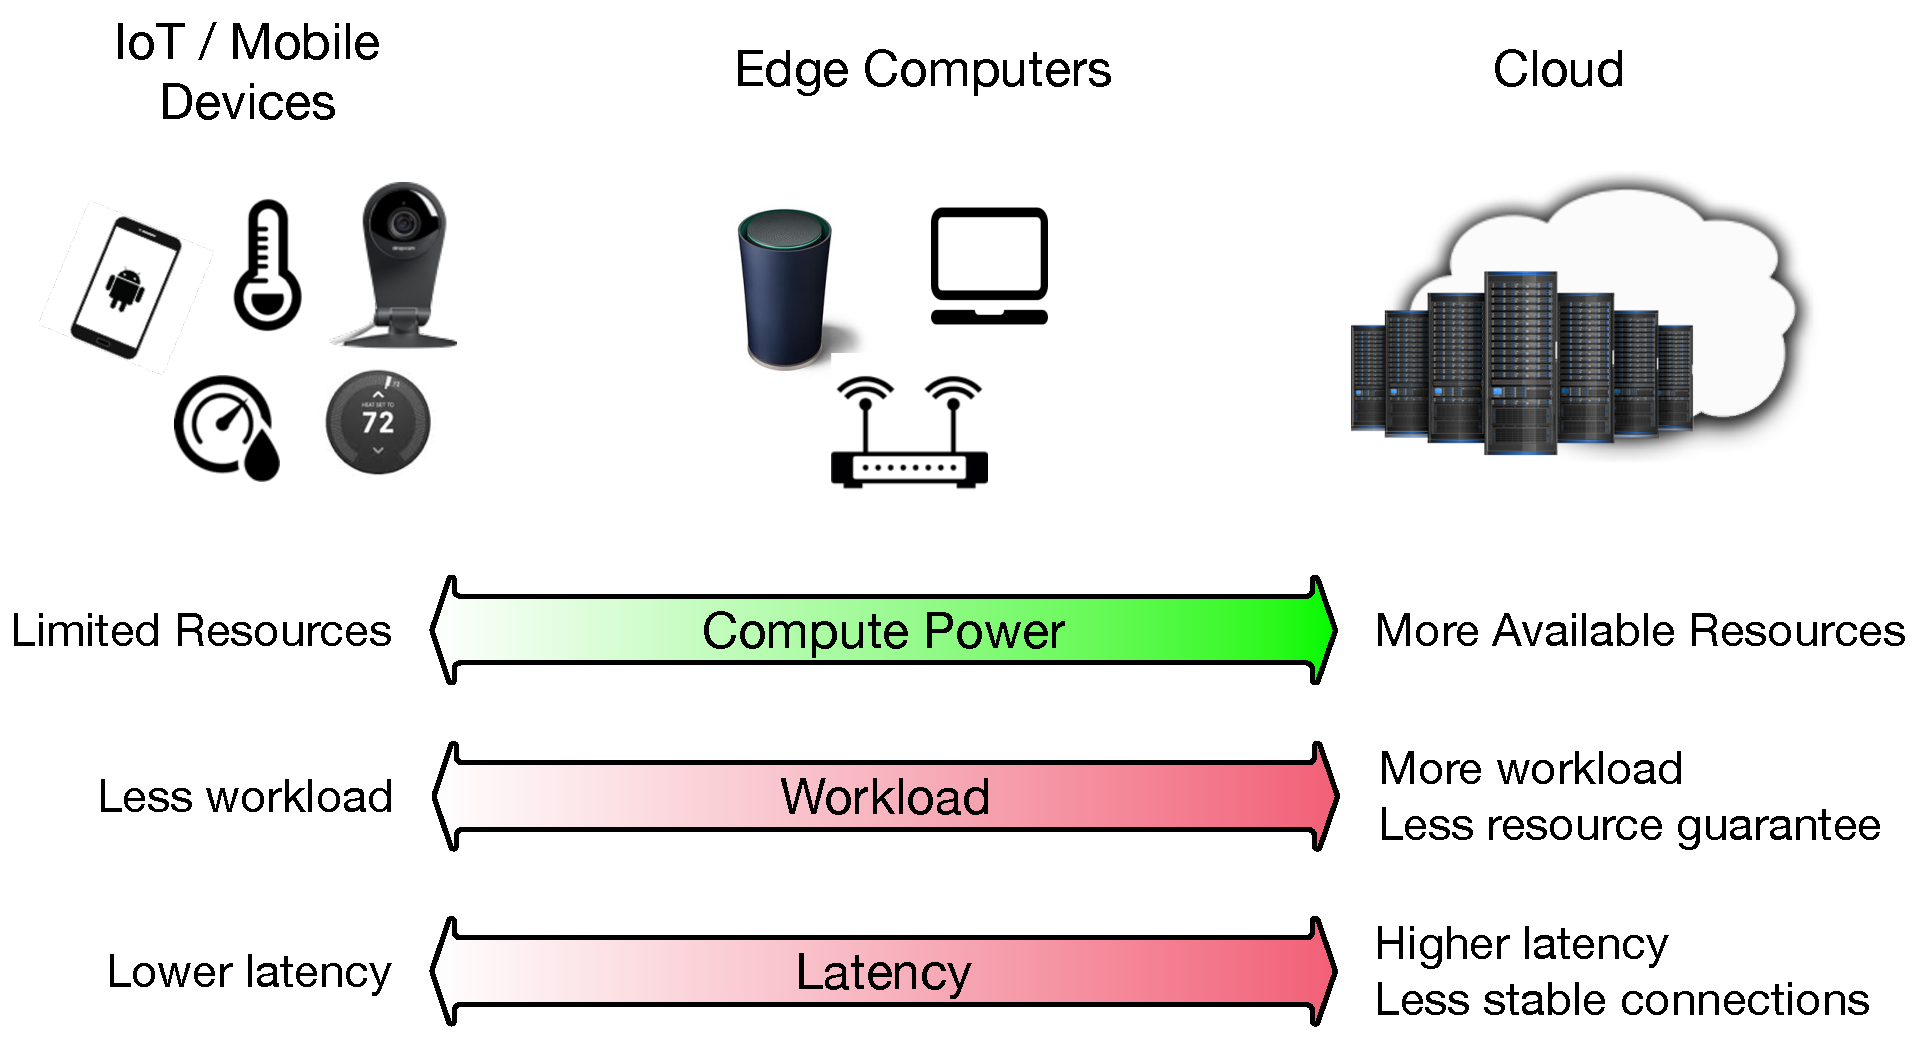
\includegraphics[width=0.85\textwidth]{figures/background.pdf}
  \caption{The characteristics of the mobile, the edge and the cloud.}
  \label{fig:edge}
\end{figure}

\autoref{fig:edge} illustrates the characteristics of the three-tier
architecture. The edge is much more powerful than end devices but less so
compared with the highly-centralized cloud. The edge serves a local area, such
as homes, buildings, or a city. As a result, it has moderate workload. The main
benefit of edge computers comes from the prime location: it sits in the middle
between IoT/mobile devices and the cloud. Applications built with the edge can
reduce network latency, keep data/information local, and tolerate cloud service
outage.

Researcher have begun to explore the benefit of edge platforms. For example, Kim
proposes an approach that leverages the edge computers as locally centralized
points for authentication and authorization to address IoT
security~\cite{kim2017securing}. Zhuo demonstrates how the edge infrastructure
can support computation offloading to achieve low
latency~\cite{chen2018application}. Mor et al.\,proposes a data-centric design
that focuses around the distribution, preservation, and protection of
information to address data privacy, scalability, durability,
etc~\cite{mor2016toward}.

While an open edge platform can realize these
benefit~\cite{zachariah1001internet}, companies tend to provide their own
gateways, such as Ninja Sphere~\cite{ninja}, SmartThings Hub~\cite{smartthings},
Wink Hub~\cite{wink}. The fact that custom gateways are an integral part of
swarm applications leads directly to ``stovepipe'' solutions or
balkanization. Data and services from one company cannot be shared or utilized
by devices from another company: connection protocols, data formats, and
security mechanisms (when present) are proprietary and often undocumented. How
to address the stovepipe issue is an active research topic. For example, Brooks
et al. proposes a component-based software architecture named ``Accessors'',
which proxies for services and things~\cite{brooks2018component}.

In addition to an open architecture, we also need to address the heterogeneous
capabilities of the edge infrastructure. As mentioned in \autoref{tab:embedded},
the swarm includes a wide spectrum of devices. It is unclear at development time
about which specific device serves as the edge. It is also difficult to make
changes to the edge, especially when it is a gateway. This is significantly from
the cloud. With its elasticity, the cloud offers the illusion of infinite
compute resources. Users can easily start another machine or even a GPU-enabled
one for heavy computation instantly. For gateways, users will need to purchase
additional devices or upgrade their existing ones: it easily takes hours or
days.

In summary, the edge offers a unique opportunity to compensate the
cloud. However, to fully realize its potentials, we need to avoid stovepipe
solutions and address challenges with the heterogeneous capabilities. This
thesis will focus on the latter.

%%% Local Variables:
%%% mode: latex
%%% TeX-master: "../background"
%%% End:


\end{document}

%%% Local Variables:
%%% mode: latex
%%% TeX-master: t
%%% End:
